% Digital Logic Report Template
% Created: 2020-01-10, John Miller

%==========================================================
%=========== Document Setup  ==============================

% Formatting defined by class file
\documentclass[11pt]{article}

% ---- Document formatting ----
\usepackage[margin=1in]{geometry}	% Narrower margins
\usepackage{booktabs}				% Nice formatting of tables
\usepackage{graphicx}				% Ability to include graphics

%\setlength\parindent{0pt}	% Do not indent first line of paragraphs 
\usepackage[parfill]{parskip}		% Line space b/w paragraphs
%	parfill option prevents last line of pgrph from being fully justified

% Parskip package adds too much space around titles, fix with this
\RequirePackage{titlesec}
\titlespacing\section{0pt}{8pt plus 4pt minus 2pt}{3pt plus 2pt minus 2pt}
\titlespacing\subsection{0pt}{4pt plus 4pt minus 2pt}{-2pt plus 2pt minus 2pt}
\titlespacing\subsubsection{0pt}{2pt plus 4pt minus 2pt}{-6pt plus 2pt minus 2pt}

% ---- Hyperlinks ----
\usepackage[colorlinks=true,urlcolor=blue]{hyperref}	% For URL's. Automatically links internal references.

% ---- Code listings ----
\usepackage{listings} 					% Nice code layout and inclusion
\usepackage[usenames,dvipsnames]{xcolor}	% Colors (needs to be defined before using colors)

% Define custom colors for listings
\definecolor{listinggray}{gray}{0.98}		% Listings background color
\definecolor{rulegray}{gray}{0.7}			% Listings rule/frame color

% Style for Verilog
\lstdefinestyle{Verilog}{
	language=Verilog,					% Verilog
	backgroundcolor=\color{listinggray},	% light gray background
	rulecolor=\color{blue}, 			% blue frame lines
	frame=tb,							% lines above & below
	linewidth=\columnwidth, 			% set line width
	basicstyle=\small\ttfamily,	% basic font style that is used for the code	
	breaklines=true, 					% allow breaking across columns/pages
	tabsize=3,							% set tab size
	commentstyle=\color{gray},	% comments in italic 
	stringstyle=\upshape,				% strings are printed in normal font
	showspaces=false,					% don't underscore spaces
}

% How to use: \Verilog[listing_options]{file}
\newcommand{\Verilog}[2][]{%
	\lstinputlisting[style=Verilog,#1]{#2}
}




%======================================================
%=========== Body  ====================================
\begin{document}

\title{ELC 2137 Lab 02: Transistor Logic Gates}
\author{Kyra Rose}

\maketitle


\section*{Summary}

  The purpose of this lab was to learn how to build logic gates using transistors. The transistors act like switches that control the voltage. After completing this lab I found that the final gate is an AND gate. This shows that we can use transistors and resistors to turn one logic gate into another (i.e Nor gate into an AND gate). 


\section*{Q\&A}

1) Which Logic Operation does the final gate implement?

The final gate implements the AND operator, therefore it is an AND gate. 

\section*{Code}

\begin{lstlisting}[style=Verilog,
	caption=Code Written for Tables and Figures 
	label=code:ex 
	]
\begin{table}[h]\centering
	\caption{Final Gate Truth table}
	\begin{tabular}{cc|c}
		\toprule
		A & B & AND \\
		\midrule
		0 & 0 & 0 \\
		0 & 1 & 0 \\
		1 & 0 & 0 \\
		1 & 1 & 1 \\
		\bottomrule
	\end{tabular} 
\end{table}
\begin{figure}[ht]\centering
	\includegraphics[width = 5in,trim = 1in 6.5in 0in 4in,clip]{demo page 1}
	
	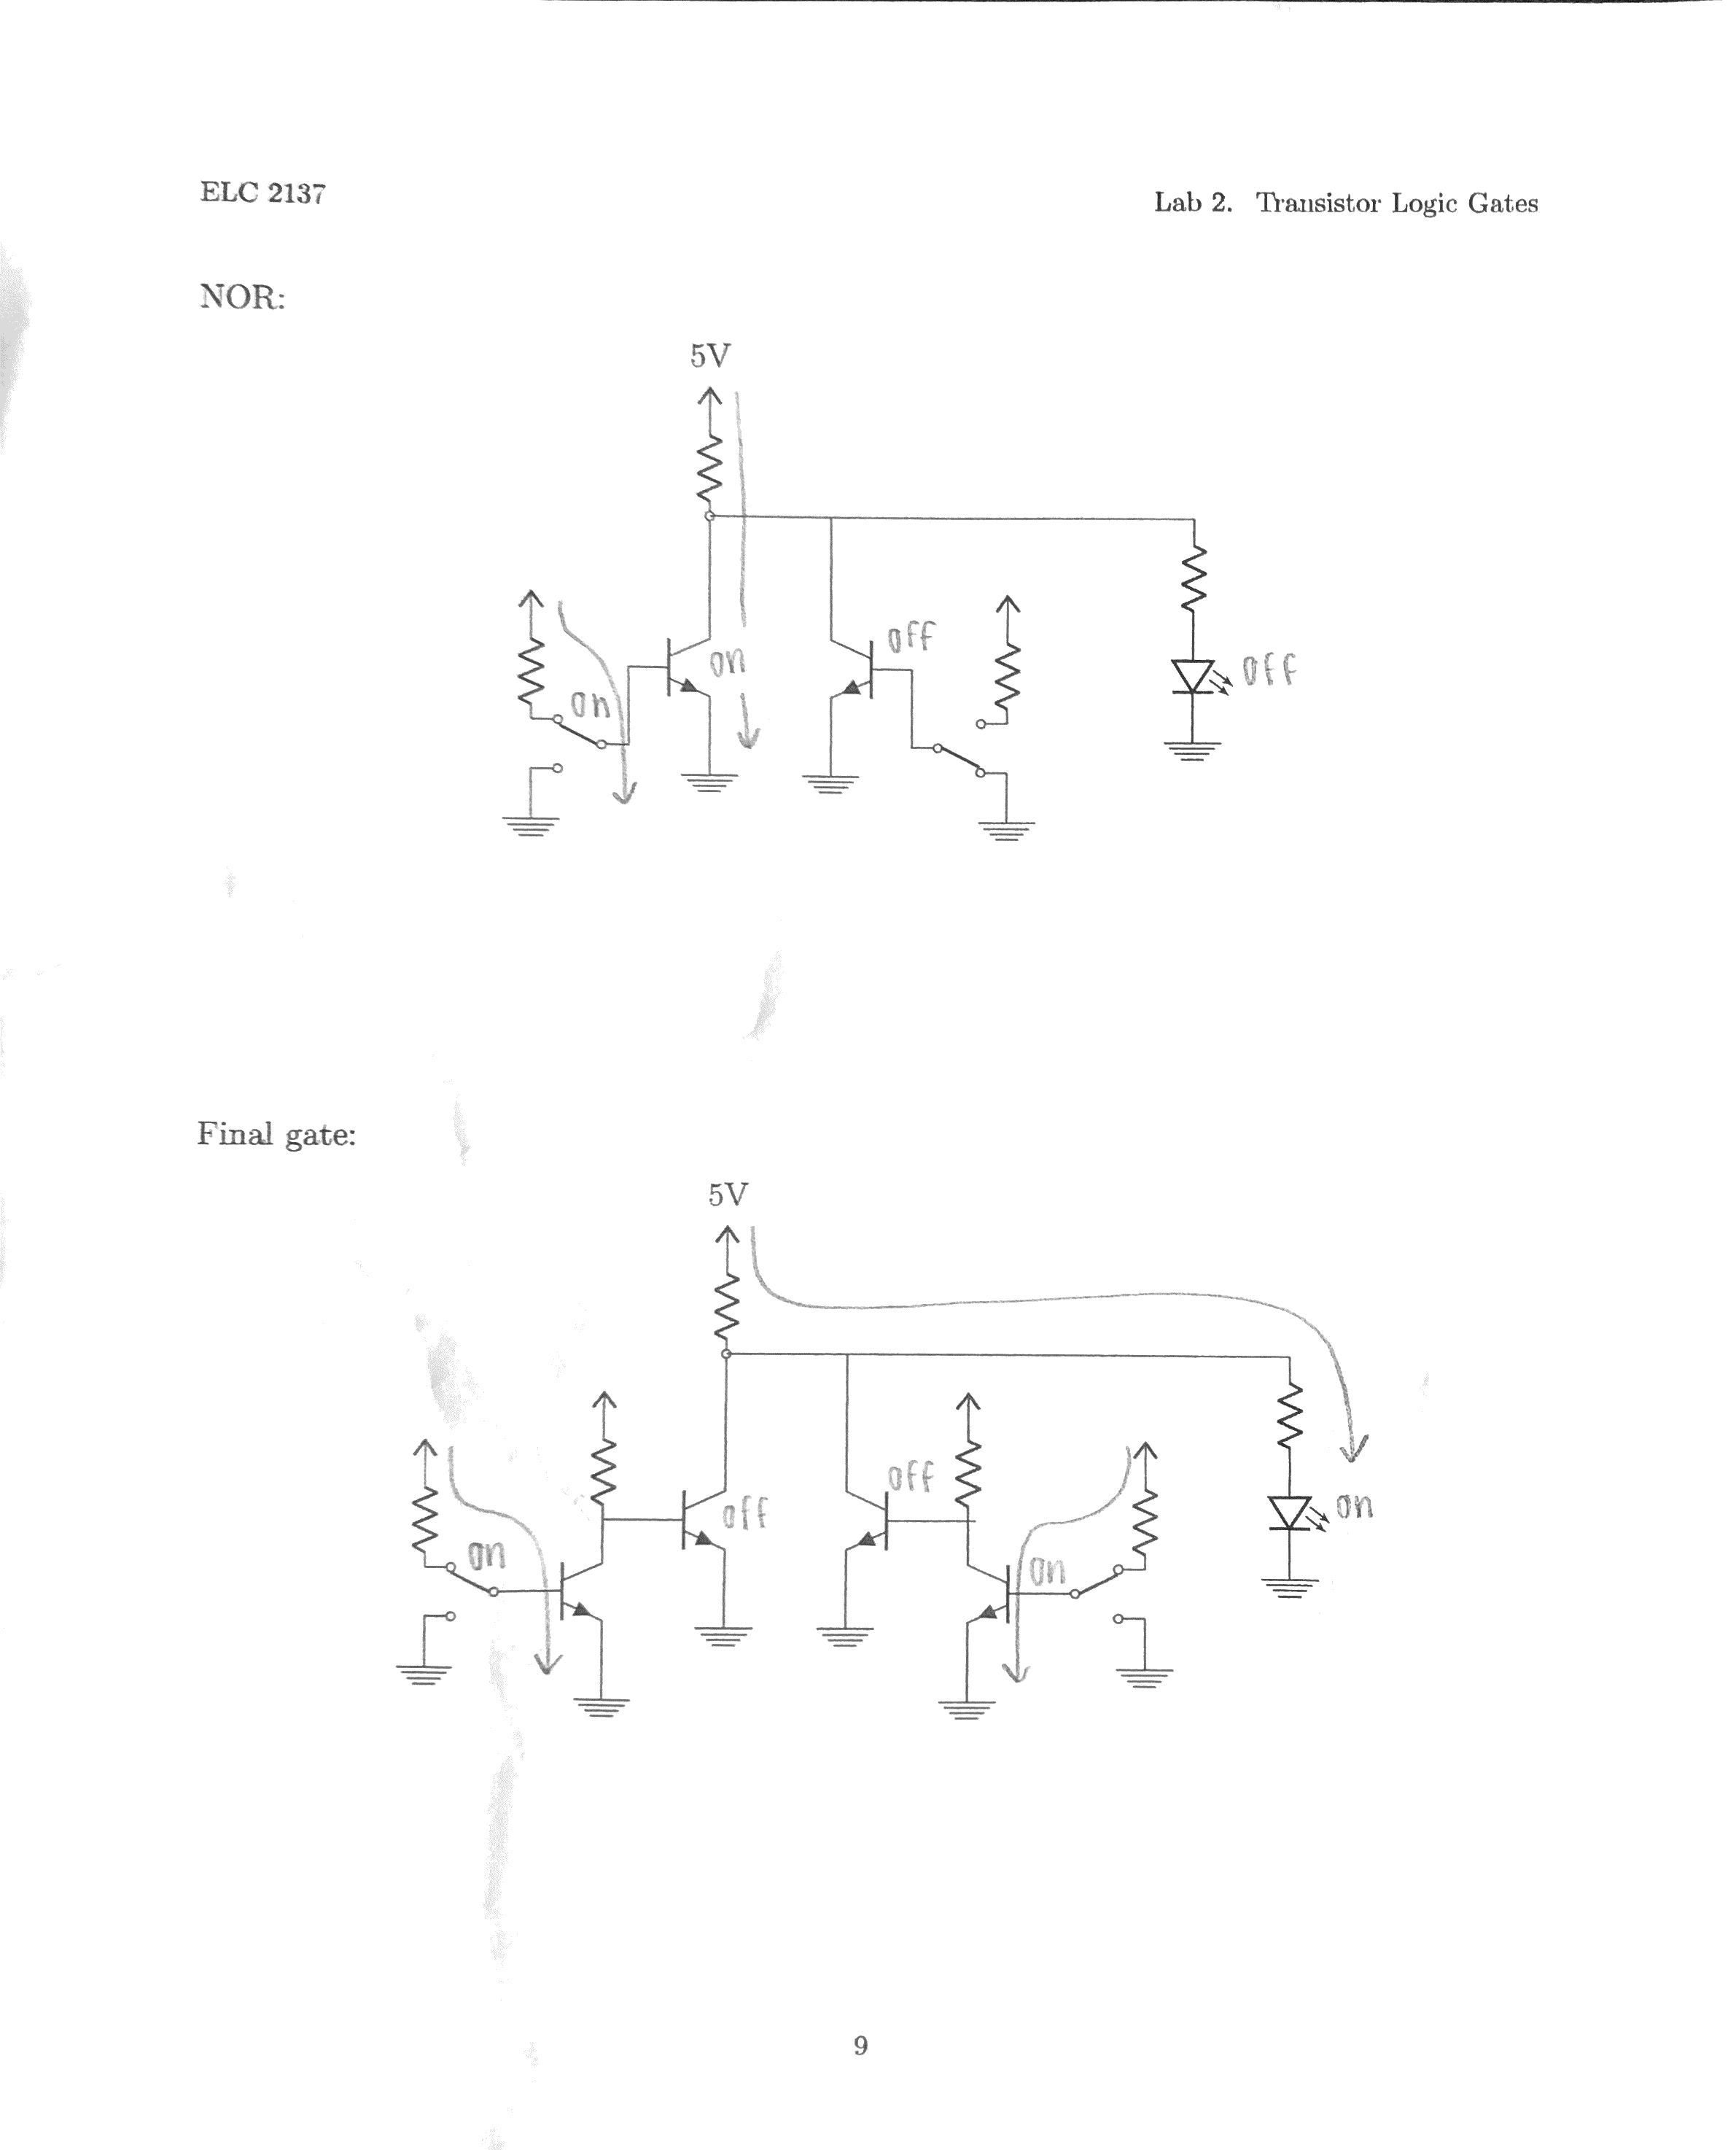
\includegraphics[width = 5in,trim = 1in 1in 0in 3.2in,clip]{demo page 2}
\end{lstlisting}


\section*{Results}

\begin{table}[h]\centering
	\caption{Final Gate Truth table}
	\begin{tabular}{cc|c}
		\toprule
		A & B & AND \\
		\midrule
		0 & 0 & 0 \\
		0 & 1 & 0 \\
		1 & 0 & 0 \\
		1 & 1 & 1 \\
		\bottomrule
	\end{tabular} 
\end{table}
\begin{figure}[ht]\centering
\includegraphics[width = 5in,trim = 1in 6.5in 0in 4in,clip]{demo page 1}

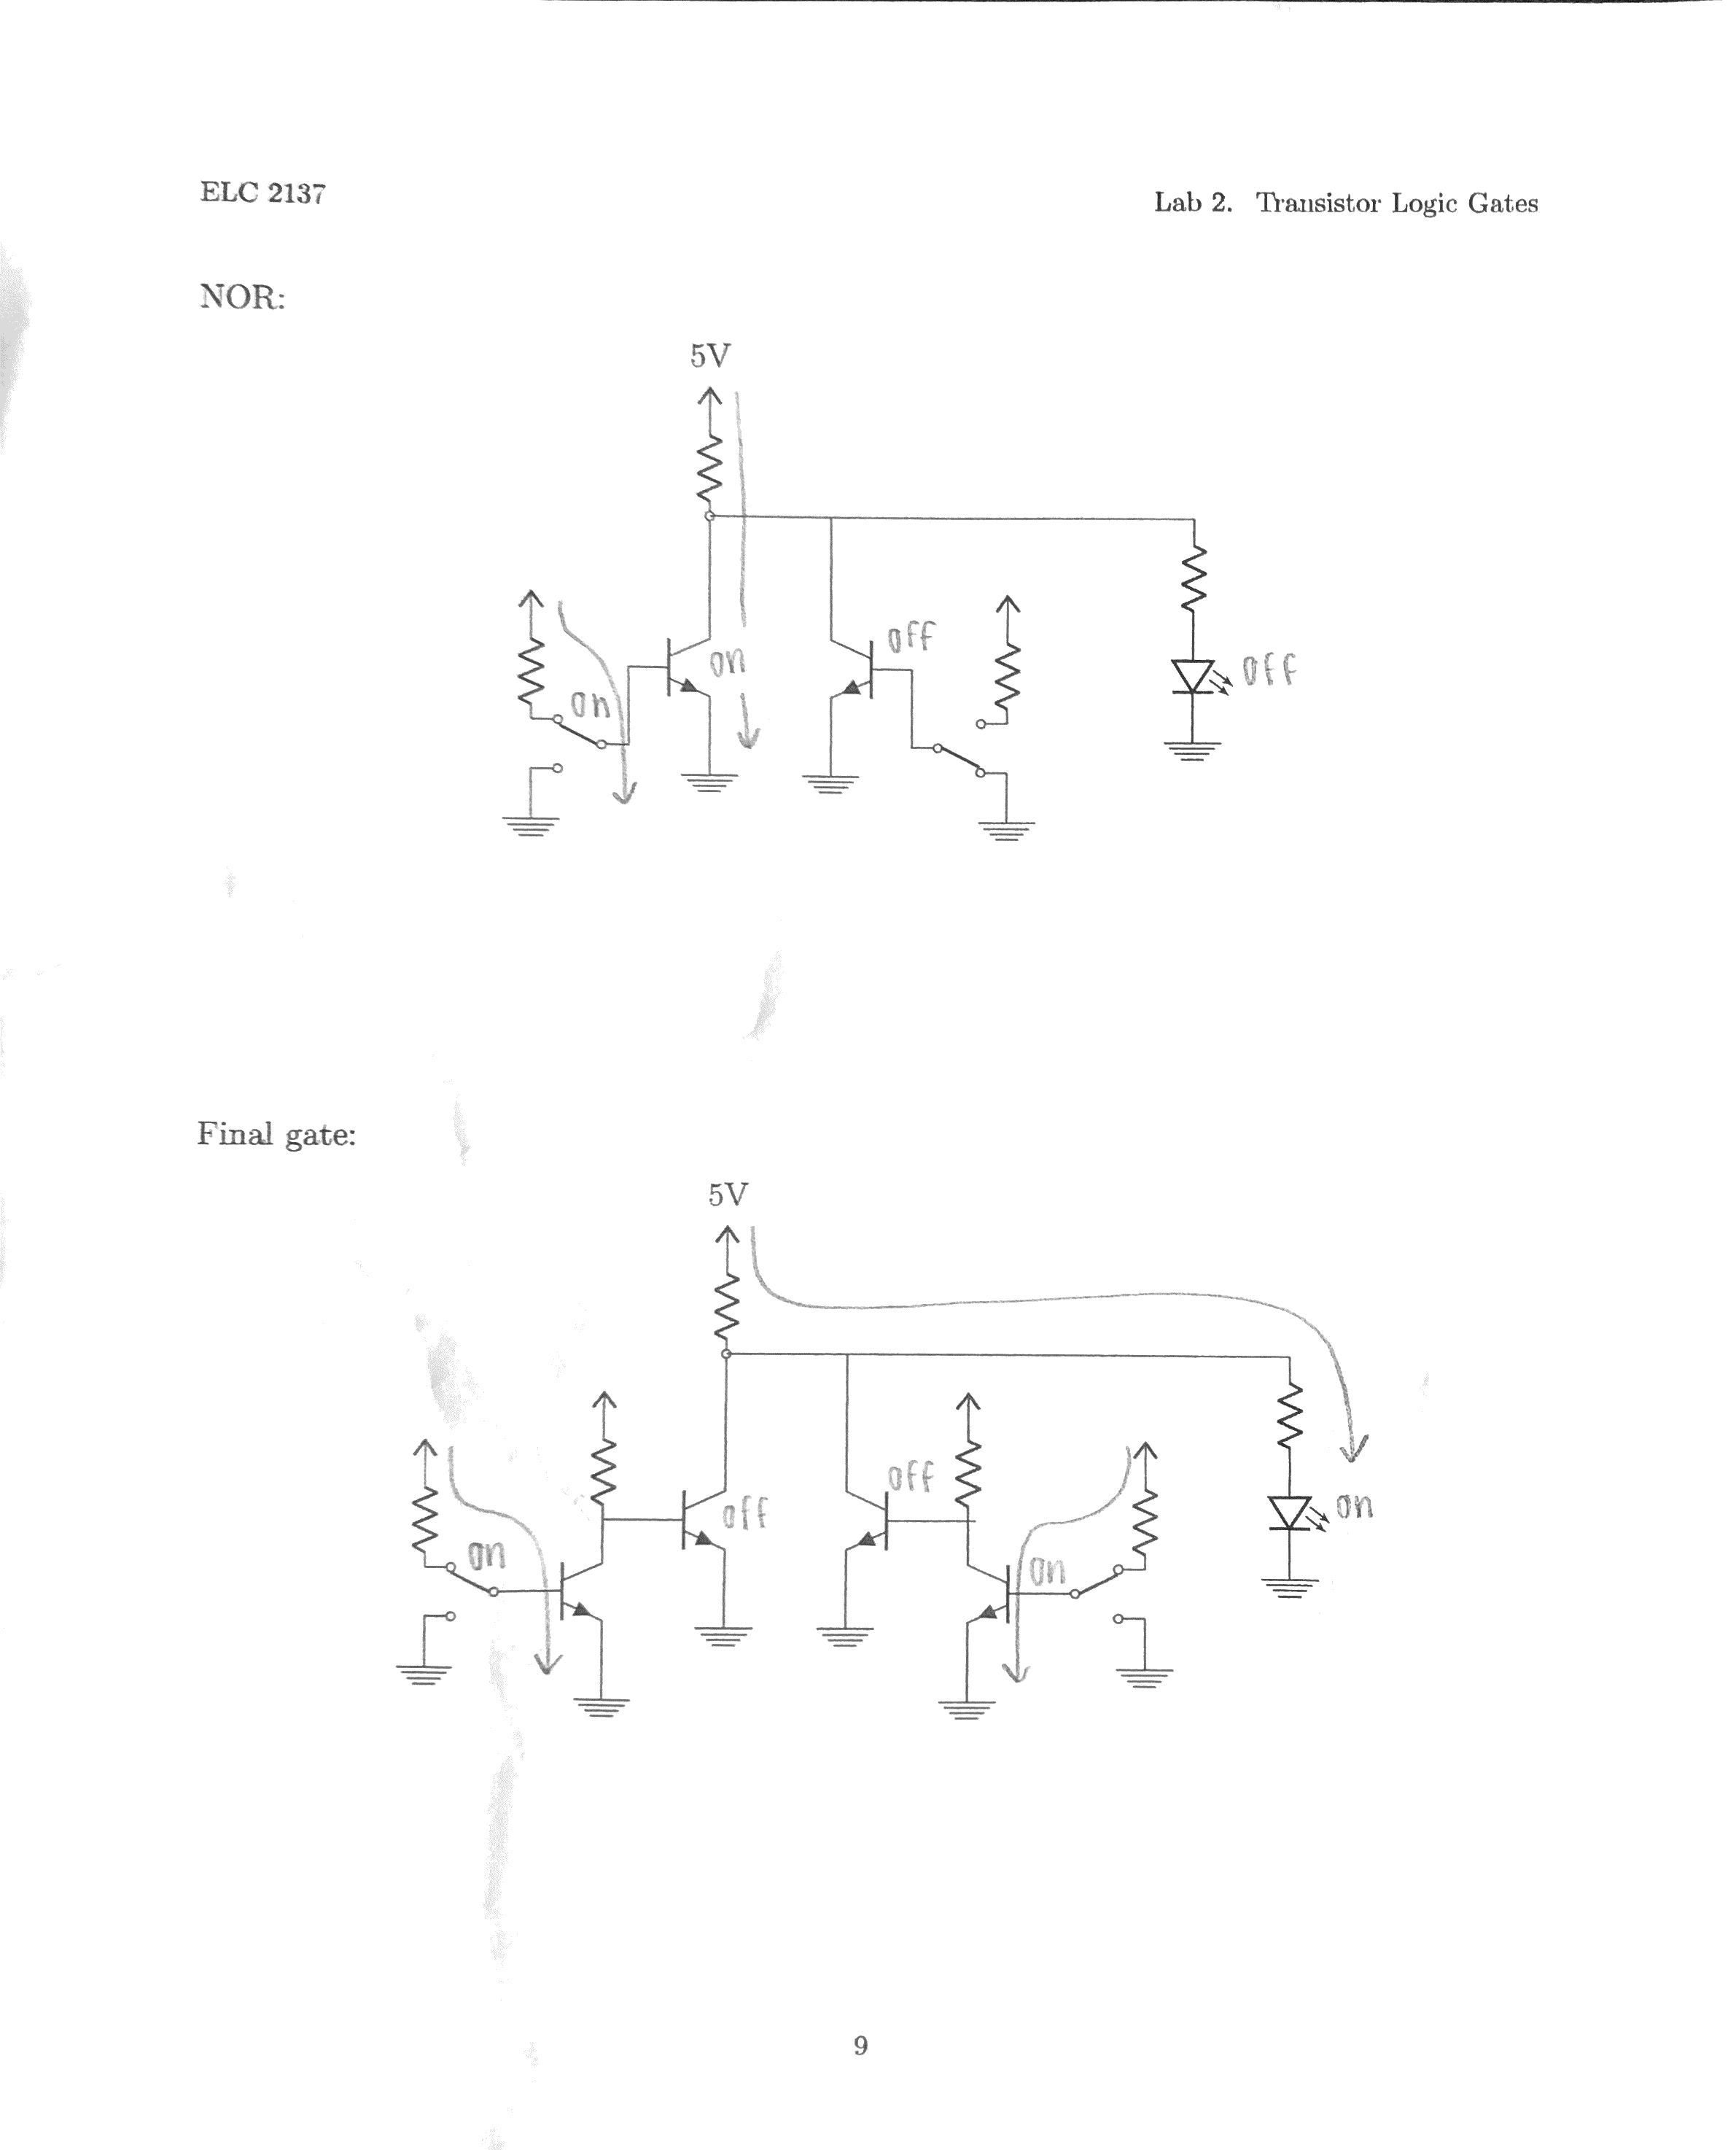
\includegraphics[width = 5in,trim = 1in 1in 0in 3.2in,clip]{demo page 2}

\end{figure}

\end{document}
